\section{Theorie}

Ein Lock-In-Verstärker wird verwendet um stark verrauschte Signale zu detektieren.
Dazu muss die Referenzfrequenz allerdings bekannt sein.

Der Aufbau eines Lock-In-Verstärkers ist in Abbildung (\ref{abb:1}) schematisch
dargestellt. Zunächst geht das Nutzsignal $U_\text{sig}$ durch einen Bandpassfilter,
welcher die Rauschanteile die eine höhere oder niedrigere Frequenz als die
Referenzfrequenz haben herausfiltert. Der Bandpassfilter ist nicht genau, wodurch
eine Bandbreite an Frequenzen übrig bleibt.

Daraufhin wird das gefilterte Nutzsignal in einem Mischer gemischt, mit einem
Referenzsignal $U_\text{ref}$ was die Referenzfrequenz als Frequenz hat. Dabei werden
die beiden mathematischen Funktionen der Signale multipliziert. Beim Mischen kommt
es darauf an ob die beiden Signale in Phase sind oder Phasenverschoben sind.

Zuletzt geht das gemischte Signal durch einen Tiefpass. Ein Tiefpass kann unter der
Vorraussetzung $RC >> \frac{1}{\omega_0}$ als Integrator wirken. Diese Vorraussetzung ist
beim Lock-In-Verstärker gegeben. Durch das Integrieten ergibt sich für das Ausgangssignal

\begin{equation}
  U_{\text{out}} = A U_0 \cos(\phi).
  \label{eq:1}
\end{equation}

Dabei ist \phi die Phasenverschiebung zwischen $U_\text{sig}$ und $U_\text{ref}$. Für den
Spezialfall, dass $U_\text{sig}$ und $U_\text{ref}$ sinusförmig sind ergibt sich Gleichung
(\ref{eq:1}) zu

\begin{equation*}
  U_{\text{out}} =  \frac{U_0}{2} \cos(\phi).
\end{equation*}

Mit dem Tiefpass am Ende lässt sich die Bandbreite des Restrauschens einstellen, indem
die Zeitkonstante $RC$ groß gemacht wird, denn es gilt die Beziehung $\Delta \nu = \frac{1}{\pi RC}$.

\begin{figure}[H]
  \centering
  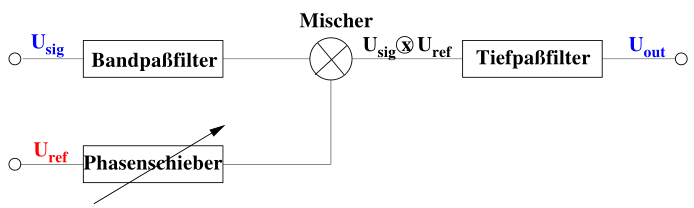
\includegraphics[width=\textwidth]{Skizze.png}
  \caption{Schematischer Aufbau eines Lock-In-Verstärkers \cite{1}.}
  \label{abb:1}
\end{figure}
